
\noindent {\color{special}{\Large \bf Para o professor}}
\vspace{.5cm}

Nesta seção, serão estudadas as frações com numeradores diferentes de 1, tanto as próprias (caso em que o numerador é menor do que ou igual ao denominador) como as impróprias (caso em que o numerador é maior do que o denominador).
Também serão abordadas a notação simbólica de frações e a comparação entre frações que tenham o mesmo denominador. 

As frações com numerador diferente de 1 são apresentadas a partir da {\bf justaposição de frações unitárias com mesmo denominador ou simplesmente contando-se essas frações}. Para isso, tem-se a representação pictórica como um apoio importante. 

Por exemplo, na atividade 1, as imagens da barra de chocolate amparam a compreensão da fração $\frac{2}{3}$ como a adição por justaposição de duas partes correspondentes à terça parte (ou à fração $\frac{1}{3}$) da barra de chocolate.

Nesse sentido, nas primeiras atividades, há um esforço deliberado para que o estudante faça uso da linguagem de frações apresentada na Lição 1 para expressar frações não unitárias. Por exemplo, na atividade 2, sabendo que uma das três fatias iguais em que foi repartida uma torta é um terço da torta, espera-se que o aluno use a linguagem ``dois terços'' ou ``dois um terços'' da torta para se referir às duas fatias. Dessa forma, ``dois terços'' são obtidos pela justaposição de duas partes correspondentes a ``um terço''. O objetivo é que esse processo se estenda para a compreensão das demais frações não unitárias. Assim, por exemplo, as frações ``quatro quintos'' e ``seis quintos'' são entendidas como ``quatro um quintos'' e ``seis um quintos'', respectivamente.

Um cuidado especial recomendado ao professor é com as frações impróprias, introduzidas logo nas primeiras atividades ainda sem notação simbólica. Não é indicado atrasar muito a introdução deste tipo de fração porque o estudante pode fixar-se na ideia de que não há fração maior do que a unidade  (por exemplo, a fração $\frac{4}{3}$ pode não fazer sentido para o estudante porque, para ele, não faz sentido dividir uma torta em 3 pedaços e tomar 4). No entanto, decidiu-se omitir do estudante as terminologias ``fração própria'' e ``fração imprópria'' por acreditar que esta linguagem é desnecessária para ele e ela pode desviar a atenção dos temas que realmente importam.

Apesar de esta lição introduzir a linguagem simbólica de frações, o estudante ainda não precisa ter um significado para a fração $\frac{a}{b}$ sem uma unidade concreta explícita: Por exemplo, ``$\frac{a}{b}$ de uma pizza'' ou ``$\frac{a}{b}$ de uma barra de chocolate''. Apenas na próxima lição, $\frac{a}{b}$ será tratado como número, requerendo do aluno a abstração que o conceito de número exige
\vspace{.15cm}

\noindent OBJETIVOS ESPECÍFICOS DA LIÇÃO 2:
\vspace{.15cm}

\noindent O aluno deve ser capaz de:
\begin{itemize}
 \item Reconhecer frações não unitárias (próprias e impróprias) como a justaposição de partes correspondentes às frações unitárias,  
  \item  Utilizar as linguagens verbal e simbólica de frações para se referir a uma fração $\frac{a}{b}$.
  \item  Reconhecer e nomear os termos de uma fração.
  \item  Comparar frações com o mesmo denominador.
  \item  Reconhecer que uma mesma quantidade pode ser expressa por frações diferentes dependendo da unidade escolhida.
\end{itemize}



\begin{multicols}{2}


\subsection{Atividade 1}

  \noindent {\bf Objetivos específicos: Levar o aluno a} \vspace{.1cm}

  \begin{itemize} %s
    \item       Estender o uso de frações para expressar quantidades que correspondam a mais do que uma fração unitária, a partir da justaposição de duas ou mais partes correspondentes às frações unitárias de mesmo denominador.
    \item       Reconhecer e usar frações para expressar quantidades que correspondam a mais do que uma fração unitária, em situação de equipartição de mais do que uma unidade (no caso, duas).
    \item       Reconhecer a necessidade de apresentar uma expressão verbal que identifique a quantidade correspondente à justaposição (ou à reunião) de duas ou mais partes correspondentes às frações unitárias de mesmo denominador.
    \item       Compreender e usar a expressão       ``$n$ terços de''       como forma de registrar a       $n$       partes da equipartição da unidade em três partes (no caso, dois terços).
    \item       Identificar a fração       ``$n$ terços de''       em uma situação de equipartição de mais do que uma unidade.
\end{itemize} %s


  \vspace{.1cm} 
  
  \noindent {\bf Recomendações e sugestões para o desenvolvimento da atividade:}\vspace{.1cm}
  
\begin{itemize} %s
    \item       Recomenda-se que a atividade seja desenvolvida em grupos de 3 a 5 alunos.
    \item       A escolha de iniciar o assunto com um problema de divisão partitiva, no lugar do contexto parte-todo, se deve a dois motivos: (1) mantém-se a questão motivadora de equipartição iniciada na lição anterior (agora com múltiplas cópias da unidade) e (2) na divisão partitiva, frações cujo numerador é maior do que o denominador (frações impróprias) fazem sentido e aparecem naturalmente, algo que pode não ocorrer no contexto parte-todo (não parece natural nomear uma parte       ``maior''       do que o todo).
    \item       As diversas soluções apresentadas pelos diferentes grupos devem ser discutidas com a turma inteira.
    \item       É possível que os alunos utilizem expressões variadas para nomear as partes dos chocolates em cada divisão e para a quantidade de chocolate que cada irmão recebeu. Por exemplo,       ``dois dos seis pedaços''      ,       ``dois pedaços de um terço de chocolate''      , dentre outras. É importante que a discussão conduza os alunos ao uso de terços:       ``dois terços'',       ``quatro terços'',       ``seis terços'', etc. Observa-se que o uso de       ``sextos''       para nomear as partes não é esperada para as perguntas que envolvem fração       ``de uma barra''       e muito povravelmente indicam uma confusão do aluno em relação ao reconhecimento da unidade. Verifique.
    \item       Nesta atividade, é importante que os alunos possam ter cópias de figuras ilustrativas das barras de chocolate para dividir e poder avaliar e decidir as suas respostas. Faça cópias das páginas para reprodução (veja no final deste livro).
\end{itemize} %s


  Classificações:
\begin{itemize} %s
    \item       Heid et al.: Conceito: identificar e descrever
    \item       Nicely, Jr.: Nível 1: reconhecer
    \item       UERJ: Observar: identificar e reconhecer
\end{itemize} %s

\begin{resposta*}{Atividade 1}
\begin{enumerate} [\quad a)] %d
    \item       Um terço.
    \item       Sim, pois a divisão foi justa no sentido de cada irmã ter recebido a mesma quantidade de chocolate.
    \item       Sim, pois cada irmã recebeu dois pedaços que equivalem, cada um, a um terço de uma barra de chocolate.
    \item       Dois terços de uma barra.
    \item       Três terços de uma barra, ou seja, uma barra inteira de chocolate.
    \item       Quatro terços de uma barra, ou seja, uma barra inteira e um terço de chocolate.
\end{enumerate} %d

\end{resposta*}


\subsection{Atividade 2}

  \noindent {\bf Objetivos específicos: Levar o aluno a} \vspace{.1cm}

  \begin{itemize} %s
    \item       Estender o uso de frações para expressar quantidades que correspondam a mais do que uma fração unitária  a partir da justaposição de duas ou mais frações unitárias de mesmo denominador.
    \item       Reconhecer a necessidade de apresentar uma expressão verbal que identifique a quantidade correspondente à justaposição de duas ou mais partes correspondentes às frações unitárias de mesmo denominador.
    \item       Reconhecer e usar frações para expressar quantidades que correspondam a mais do que uma fração unitária em situação de equipartição de mais do que uma unidade (no caso, três).
    \item       Compreender e usar a expressão       ``$n$ quintos de''       como forma de identificar a quantidade equivalente a       $n$       partes da equipartição da unidade em quintos, incluindo os casos em que       $n$       é maior do que cinco (frações impróprias).
    \item       Analisar uma situação de comparação de frações com o mesmo denominador.
\end{itemize} %s


  \vspace{.1cm}
  
  \noindent {\bf Recomendações e sugestões para o desenvolvimento da atividade:}\vspace{.1cm}

  \begin{itemize} %s
    \item       Recomenda-se que a atividade seja desenvolvida em grupos de 3 a 5 alunos.
    \item       As diversas soluções apresentadas pelos diferentes grupos devem ser discutidas com a turma inteira.
    \item       Em particular, no Item a), não se espera, nem se recomenda, que a representação feita pelos alunos seja amparada pela medida. O objetivo é que façam a equipartição livremente e de forma coerente. Assim, por exemplo, pode ser aceita como resposta a solução indicada na figura a seguir.
\end{itemize} %s

\noindent \begin{tikzpicture}[scale=.4, x=1mm,y=1mm, rotate=90]
 \draw (0,0) rectangle (30,60);
 \foreach \x in {12,24,...,48} \draw (0,\x) -- (30,\x);
 \node[rotate=90, attention] at (15,54) {{\tiny Amarildo}};
 \node[rotate=90, attention] at (15,42) {{\tiny Beto}};
 \node[rotate=90, attention] at (15,30) {{\tiny Carlos}};
 \node[rotate=90, attention] at (15,18) {{\tiny Davi}};
 \node[rotate=90, attention] at (15,6) {{\tiny Edison}};
\end{tikzpicture}
\begin{tikzpicture}[scale=.4, x=1mm,y=1mm, rotate=90]
 \draw (0,0) rectangle (30,60);
 \foreach \x in {12,24,...,48} \draw (0,\x) -- (30,\x);
 \node[rotate=90, attention] at (15,54) {{\tiny Amarildo}};
 \node[rotate=90, attention] at (15,42) {{\tiny Beto}};
 \node[rotate=90, attention] at (15,30) {{\tiny Carlos}};
 \node[rotate=90, attention] at (15,18) {{\tiny Davi}};
 \node[rotate=90, attention] at (15,6) {{\tiny Edison}};
\end{tikzpicture}
\begin{tikzpicture}[scale=.4, x=1mm,y=1mm, rotate=90]
 \draw (0,0) rectangle (30,60);
 \foreach \x in {12,24,...,48} \draw (0,\x) -- (30,\x);
 \node[rotate=90, attention] at (15,54) {{\tiny Amarildo}};
 \node[rotate=90, attention] at (15,42) {{\tiny Beto}};
 \node[rotate=90, attention] at (15,30) {{\tiny Carlos}};
 \node[rotate=90, attention] at (15,18) {{\tiny Davi}};
 \node[rotate=90, attention] at (15,6) {{\tiny Edison}};
\end{tikzpicture}

\begin{itemize} %s
    \item       Em suas respostas, é possível que os alunos utilizem expressões variadas para nomear as partes das tortas em cada divisão e para as quantidades de torta que cada irmão recebe. Por exemplo,       ``três dos quinze pedaços''      ,       ``três pedaços de um quinto de torta''      , dentre outras. É importante que a discussão conduza os alunos ao uso de quintos:       ``três quintos''      ,       ``seis quintos''      ,       ``quinze quintos''      , etc.
    \item       Espera-se que, no final da atividade, o aluno tome conhecimento e reconheça o significado das expressões dois quintos e três quintos, mesmo que não o faça espontaneamente (usando, por exemplo, especificações como       ``dois pedaços''       ou       ``duas fatias'') e seja necessária a intervenção do professor. O professor deve fazer e incentivar o uso da terminologia de frações que se quer estabelecer nesta lição.
    \item       Nesta atividade, é importante que os alunos possam ter cópias de figuras ilustrativas da torta para dividir e poder avaliar e decidir suas respostas. Faça cópias das páginas para reprodução do final do livro.
    \item       Nos Itens c) e d), não basta uma resposta       ``Sim''       ou       ``Não''      . É importante estimular os seus alunos a darem uma justificativa.
\end{itemize} %s



  Classificações
\begin{itemize} %s
    \item       Heid et al.: Conceito: identificar, descrever
    \item       Nicely, Jr.: Nível 1: reconhecer
    \item       UERJ: Observar: identificar, reconhecer
\end{itemize} %s

  Itens c) e d)
\begin{itemize} %s
    \item       Heid et al.: Raciocínio: justificar
    \item       Nicely, Jr.: Nível 6: justificar
    \item       UERJ: Avaliar: julgar
\end{itemize} %s

\begin{resposta*}{Atividade 2}
\begin{enumerate} [\quad a)] %d
    \item       Uma resposta possível (entre várias): dividir cada uma das três tortas em 5 partes iguais e, então, com as 15 partes disponíveis, distribuir 3 partes para cada amigo, como mostra a figura a seguir      
\begin{center}    
\begin{tikzpicture}[scale=.4, x=1mm,y=1mm, rotate=90]
 \draw (0,0) rectangle (30,60);
 \foreach \x in {12,24,...,48} \draw (0,\x) -- (30,\x);
 \node[rotate=90, attention] at (15,54) {{\tiny Amarildo}};
 \node[rotate=90, attention] at (15,42) {{\tiny Beto}};
 \node[rotate=90, attention] at (15,30) {{\tiny Carlos}};
 \node[rotate=90, attention] at (15,18) {{\tiny Davi}};
 \node[rotate=90, attention] at (15,6) {{\tiny Edison}};
\end{tikzpicture}
\end{center}
    \item
\begin{enumerate}[I)]
          \item Três quintos.
          \item Seis quintos (ou uma torta inteira e um quinto de torta).
          \item Nove quintos.
          \item Doze quintos (ou duas tortas inteiras e dois quintos de torta).
          \item Quinze quintos (ou três tortas inteiras).
\end{enumerate}

    \item       A quantidade de torta que cada amigo recebeu não pode ser menor do que um quinto de torta pois se isto acontecesse, a quantidade total de torta recebida pelos três amigos seria menor do que cinco quintos de torta, isto é, seria menor do que uma torta inteira, o que não é o caso. Um argumento análogo mostra que a quantidade de torta que cada amigo recebeu não pode ser menor do que dois quintos de torta.
    \item       A quantidade de torta que cada amigo recebeu não pode ser maior do que três quintos de torta pois se isto acontecesse, a quantidade total de torta recebida pelos três amigos seria maior do que quinze quintos de torta, isto é, seria maior do que três tortas inteiras, o que não é o caso. Um argumento análogo mostra que a quantidade de torta que cada amigo recebeu não pode ser maior do que quatro quintos de torta.
\end{enumerate} %d


\end{resposta*}


  

\subsection{Atividade 3}

  \noindent {\bf Objetivos específicos: Levar o aluno a} \vspace{.1cm}
  
\begin{itemize} %s
    \item       Estender o uso de frações para expressar quantidades que correspondam a mais do que uma fração unitária, a partir da justaposição de duas ou mais partes correspondentes às frações unitárias de mesmo denominador.
    \item       Reconhecer e usar frações para expressar quantidades que correspondam a mais do que uma fração unitária em situação de equipartição de mais do que uma unidade (no caso, oito).
    \item       Compreender e usar a expressão       ``$n$ oitavos de''       como forma de identicar a quantidade equivalente a       $n$       partes da equipartição da unidade em oito partes, incluindo os casos em que       $n$       é maior do que oito (frações impróprias).
    \item       Reconhecer que uma mesma quantidade pode ser expressa por frações equivalentes de uma mesma unidade (por exemplo,       ``meia torta''       e       ``quatro oitavos de torta''       representam a mesma quantidade de torta).
\end{itemize} %s


  \vspace{.1cm}
  
  \noindent {\bf Recomendações e sugestões para o desenvolvimento da atividade:}\vspace{.1cm}

\begin{itemize} %s
    \item       Recomenda-se que a atividade seja desenvolvida em grupos de 3 a 5 alunos.
    \item       As diversas soluções apresentadas pelos diferentes grupos devem ser discutidas com a turma inteira.
    \item       É importante que a discussão conduza os alunos ao uso de oitavos:       ``quatro oitavos''      ,       ``dez oitavos''       e       ``uma torta e dois oitavos''      .
    \item       No entanto, cabe ressaltar que não se objetiva o uso da notação de fração mista para representar, por exemplo,       ``uma torta e dois oitavos''      .
    \item       As respostas esperadas para o Item c) podem surgir na resolução do Item b). Caso isso aconteça, recomenda-se que as frações corretas correspondentes a       $4$       fatias de torta ($\frac{1}{2}$       de torta,       $\frac{2}{4}$       de torta,       $\frac{3}{6}$       de torta, etc.) sejam reconhecidas como tal, mas que, conforme solicitado pelo enunciado, a resposta deve ser dada em termos de oitavos.
    \item       No Item c), é importante estimular o aluno a dar uma explicação para sua resposta: por que você pensou em       $\frac{1}{2}$       de torta? Por que você pensou em       $\frac{3}{6}$       de torta? Etc.
\end{itemize} %s


  Classificações
\begin{itemize} %s
    \item       Heid et al.: Conceito: identificar, descrever
    \item       Nicely, Jr.: Nível 1: reconhecer
    \item       UERJ: Observar: identificar, reconhecer
\end{itemize} %s




\begin{resposta*}{Atividade 3}
\begin{enumerate} [\quad a)] %s
    \item       Cada fatia é um oitavo de torta, pois cada torta está dividida em oito partes iguais.
    \item       Havia para a sobremesa quatro oitavos de torta.
    \item       Meia torta, pois quatro fatias de torta têm exatamente a mesma quantidade de torta que meia torta.
\end{enumerate} %s
  
  \begin{center}
  
\includegraphics[width=175pt, keepaspectratio]{../../livro/media/cap2/secoes/pngs_licao_02/ativ3_resposta.png}
  \end{center}
  
\begin{enumerate} [\quad a)] %s
    \item       Algumas respostas possíveis: dez oitavos de torta;  uma torta inteira e dois oitavos de torta; uma torta inteira e um quarto de torta.
\end{enumerate} %s

\end{resposta*}



\subsection{Atividade 4}

  \noindent {\bf Objetivos específicos: Levar o aluno a} \vspace{.1cm}
  
\begin{itemize} %s
    \item       Identificar frações do tipo       ``$n$ meios''      ,       ``$n$ terços''      , ...,       ``$n$ décimos''       em diferentes modelos visuais de frações em situações onde há uma indicação explícita da unidade.
    \item       Compreender frações do tipo       ``$n$ meios''      ,       ``$n$ terços''      , ...,       ``$n$ décimos''       como forma de identicar a quantidade equivalente a       ``$n$''       cópias da fração unitária       ``$\frac{1}{m}$''       (incluindo os casos em que       $n \geq m$      ) em siutações onde há uma indicação explícita da unidade.
\end{itemize} %s


  \vspace{.1cm}
  
  \noindent {\bf Recomendações e sugestões para o desenvolvimento da atividade:}\vspace{.1cm}

  \begin{itemize} %s
    \item       Esta atividade pode ser resolvida individualmente, mas é essencial que seja discutida com toda a turma.
    \item       Observe que, enquanto que nas atividades anteriores cópias múltiplas da unidade já estavam naturalmente disponíveis (as duas barras de chocolate na Atividade 1, as três tortas salgadas na Atividade 2, as várias tortas divididas em oito partes na confeitaria da Atividade 3), nesta atividade, o aluno deve identificar frações a partir de uma única cópia da unidade, sem qualquer subdivisão registrada. Por exemplo, no item c), o aluno deve registrar nove meios de uma estrelinha, sem a subdivisão explicitada. Assim, a atividade oferece uma oportunidade para reforçar a compreensão de frações em um contexto diferente daquele em que a parte correspondente à fração é identificada totalmente inserida em uma unidade, frequentemente já subdividida. Esse tipo de representação, muito associada ao significado parte/todo, pode limitar a compreensão de frações impróprias.
    \item       Nesta atividade, espera-se que o aluno identifique uma equipartição da unidade que defina a fração unitária       $\frac{1}{m}$       da unidade adequada à compor a parte colorida e que, então, tome a quantidade       $n$       correta desta fração unitária, mesmo no caso em que       $n > m$
\end{itemize} %s


  Classificações
\begin{itemize} %s
    \item       Heid et al.: Conceito: identificar
    \item       Nicely, Jr.: Nível 1: reconhecer
    \item       UERJ: Observar: identificar, nomear
\end{itemize} %s

\begin{resposta*}{Atividade 4}
  \begin{enumerate}[a)]
   \item dois terços.
   \item dois meios.
   \item dois quintos.
   \item nove meios.
   \item oito sextos.
\end{enumerate}
  \end{resposta*}



\subsection{Sobre o Organizando as ideias}



  Nesta etapa, espera-se que os alunos compreendam as frações   $\frac{a}{b}$   como adição por justaposição de   {\it a}   frações   $\frac{1}{b}$   da unidade. Observe que esse entendimento é construído a partir de modelos contínuos e amparado por situações concretas. Assim, como explicado na introdução desta seção, por exemplo,   ``dois terços''   de uma unidade dada são obtidos pela justaposição de duas partes correspondentes a   ``um terço''   da mesma unidade.

  Esse entendimento terá reflexos na forma como são lidas as frações   $\frac{a}{b}$  . Não se espera, nem se recomenda, que seja sugerida aos alunos a leitura de   $\frac{a}{b}$   como   ``{\it a sobre b}''   nem como   ``{\it a dividido por b}''  . Nesta etapa, espera-se que os alunos leiam essas frações, por exemplo, como   ``dois terços''   ou   ``dois um terços''   da unidade. As outras formas de leitura serão tratadas em seções posteriores.

  Nesse contexto, é importante também discutir com os alunos as frações que representam números naturais. Por exemplo, na atividade 2, a fração   $\frac{3}{3}$   da torta é a torta inteira e a fração   $\frac{6}{3}$   da torta são duas tortas.

  Por fim, observa-se que a notação de fração pode não parecer natural para os alunos, porque é um símbolo composto por dois números de significados diferentes, um sobre o outro. Isso contraria a escrita usual dos números naturais. Alguns povos antigos tiveram representações diferentes para estes números.  Contudo, é importante lembrar que hoje essa é a notação mundialmente aceita, devendo, portanto, ser bem compreendida.



\subsection{Atividade 5}

  \noindent {\bf Objetivos específicos: Levar o aluno a} \vspace{.1cm}

  \begin{itemize} %d
    \item       Comparar diversas maneiras de se representar uma fração (por extenso, simbolicamente e graficamente).
    \item       Discutir aspectos dessas representações.
\end{itemize} %d


  \vspace{.1cm} 
  
  \noindent {\bf Recomendações e sugestões para o desenvolvimento da atividade:}\vspace{.1cm}

  \begin{itemize} %d
    \item       Essa é uma atividade que o aluno pode fazer individualmente.
    \item       É possível que os alunos utilizem frações equivalentes como resposta para um mesmo item. Por exemplo, as frações       $\frac{4}{12}$      ,       $\frac{2}{6}$       e       $\frac{1}{3}$        descrevem corretamente a quantidade de pizza consumida por Pedro. Nestes casos, dê a oportunidade para que cada aluno explique como chegou à sua resposta pois, procedendo desta maneira, mesmo de forma pontual, os alunos perceberão que uma mesma quantidade pode ser descrita por frações com nomes diferentes, um preparo para o assunto       ``frações equivalentes''       que será tratado na Lição 4.
    \item       Esta atividade procura mostrar uma das qualidades da notação simbólica matemática: expressar um conceito com economia de escrita. Mas sua importância vai muito mais além: ela é uma ferramenta de pensamento que permite encapsular detalhes, simplificar procedimentos, abstrair e generalizar conceitos. Assim, é muito importante fazer com que seus alunos se familiarizem com a notação simbólica matemática para frações: ela será fundamental nas lições sobre operações com frações.
\end{itemize} %d


  Classificações
\begin{itemize} %s
    \item       Heid et al.: Produto: gerar
    \item       Nicely, Jr.: Nível 5: converter (simbolizar)
    \item       UERJ: Interpretar: discriminar
\end{itemize} %s




\begin{resposta*}{Atividade 5}


    \begin{tabular}{m{.08\textwidth}m{.08\textwidth}m{.08\textwidth}m{.08\textwidth}}
      
        \small Pedro & \small Isabella  &   \small Bernardo  &   \small Manuela  \\
      \hline
       \begin{tikzpicture}[x=1mm,y=1mm, scale=.7]
        \draw[fill=common, fill opacity=.3] (0,0) circle (10);
        \fill[attention] (90:10) arc (90:210:10) -- (0,0) -- cycle;
        \foreach \x in {0,30,...,150}\draw (\x:10) -- (\x:-10);        
       \end{tikzpicture}&
       \begin{tikzpicture}[x=1mm,y=1mm, scale=.7]
        \draw[fill=common, fill opacity=.3] (0,0) circle (10);
        \fill[attention] (210:10) arc (210:360:10) -- (0,0) -- cycle;
        \foreach \x in {0,30,...,150}\draw (\x:10) -- (\x:-10);        
       \end{tikzpicture}&
       \begin{tikzpicture}[x=1mm,y=1mm, scale=.7]
        \draw[fill=common, fill opacity=.3] (0,0) circle (10);
        \fill[attention] (0:10) arc (0:60:10) -- (0,0) -- cycle;
        \foreach \x in {0,30,...,150}\draw (\x:10) -- (\x:-10);        
       \end{tikzpicture}&
       \begin{tikzpicture}[x=1mm,y=1mm, scale=.7]
        \draw[fill=common, fill opacity=.3] (0,0) circle (10);
        \fill[attention] (60:10) arc (60:90:10) -- (0,0) -- cycle;
        \foreach \x in {0,30,...,150}\draw (\x:10) -- (\x:-10);        
       \end{tikzpicture}\\
      \hline 
      \centering  {\small quatro doze avos}  & \centering  {\small cinco doze avos}  & \centering  {\small dois doze avos}  & {\centering  {\small um doze avos}}   \\
      \hline
       \centering $\frac{4}{12}$  & \centering  $\frac{5}{12}$  & \centering  $\frac{2}{12}$   & \centering  $\frac{1}{12}$ 
    \end{tabular}

\begin{enumerate} [\quad a)] %s
    \item       A que usa a notação simbólica matemática.
    \item       As respostas podem variar de pessoa para pessoa. No entanto, a justificativa deve ser coerente com a resposta. Discuta com a turma as diferentes respostas.
\end{enumerate} %s

\end{resposta*}

\subsection{Atividade 6}

  \noindent {\bf Objetivo específico: Levar o aluno a}\vspace{.1cm}
  
\begin{itemize} %s
    \item       Comparar frações com relação a uma fração de referência (no caso, a fração       $\frac{1}{2}$      ) usando modelos de área.
\end{itemize} %s


  \vspace{.1cm} 
  
  \noindent {\bf Recomendações e sugestões para o desenvolvimento da atividade:}\vspace{.1cm}

  \begin{itemize} %s
    \item       Essa é uma atividade que o aluno pode fazer individualmente.
    \item       Incentive seus alunos a darem justificativas para suas respostas, mesmo que informais.
\end{itemize} %s


  Classificações
\begin{itemize} %s
    \item       Heid et al.: Conceito: identificar
    \item       Nicely, Jr.: Nível 3: comparar
    \item       UERJ: Observar: identificar e reconhecer; Ordenar
\end{itemize} %s

\begin{resposta*}{Atividade 6}
\begin{enumerate} [\quad a)] %s
    \item       A parte pintada é exatamente igual a       $\frac{1}{2}$       da figura.
    \item       A parte pintada é igual a       $\frac{4}{10}$       e é menor do que       $\frac{1}{2}$       da figura.
    \item       A parte pintada é igual a       $\frac{6}{10}$       e é maior do que       $\frac{1}{2}$       da figura.
\end{enumerate} %s

\end{resposta*}

\subsection{Atividade 7}

  \noindent {\bf Objetivo específico: Levar o aluno a}\vspace{.1cm}
  
\begin{itemize} %s
    \item       Comparar frações unitárias a partir de representações usando modelos circulares.
    \item       Mais especificamente, comparar um quarto e um oitavo.
\end{itemize} %s


  \vspace{.1cm} 
  
  \noindent {\bf Recomendações e sugestões para o desenvolvimento da atividade:}\vspace{.1cm}
  
\begin{itemize} %s
    \item       Esta atividade pode ser resolvida individualmente, mas é essencial que seja discutida com toda a turma.
    \item       Em particular, incentive os alunos a argumentar, justificando a sua resposta.
    \item       Coduza a discussão de modo a que consigam reconhecer que quanto maior o denominador, menor a fração.
\end{itemize} %s


  Classificações:
\begin{itemize} %s
    \item       Heid et al.: Conceito: gerar
    \item       Nicely, Jr.: Nível 3: comparar
    \item       UERJ: Observar: Observar: identificar e reconhecer; Ordenar
\end{itemize} %s



\begin{resposta*}{Atividade 7}
\begin{enumerate} [\quad a)] %s
    \item             $\frac{1}{4}$      .
    \item             $\frac{1}{8}$      .
    \item       Uma fatia da primeira pizza tem mais quantidade que uma fatia da segunda pizza: precisamente, o dobro da quantidade. Isto acontece porque são necessárias duas fatias da segunda pizza para ter-se a mesma quantidade de pizza que uma fatia da primeira pizza, como mostra o desenho a seguir.
\end{enumerate} %s
\begin{center}
       \begin{tikzpicture}[x=1mm,y=1mm, scale=.7]
        \draw[fill=common, fill opacity=.3] (0,0) circle (10);
        \fill[attention] (180:10) arc (180:270:10) -- (0,0) -- cycle;
        \foreach \x in {0,90}\draw (\x:10) -- (\x:-10);        
       \end{tikzpicture} \quad \quad
       \begin{tikzpicture}[x=1mm,y=1mm, scale=.7]
        \draw[fill=common, fill opacity=.3] (0,0) circle (10);
        \fill[attention] (180:10) arc (180:270:10) -- (0,0) -- cycle;
        \foreach \x in {0,45,90, 135}\draw (\x:10) -- (\x:-10);        
       \end{tikzpicture} 
\end{center}
\end{resposta*}





\subsection{Atividade 8}


  \noindent {\bf Objetivos específicos: Levar o aluno a} \vspace{.1cm}:

  \begin{itemize} %s
    \item       Reconhecer que uma mesma quantidade pode ser expressa por frações diferentes dependendo da unidade escolhida.
    \item       Utilizar linguagem simbólica para se referir a uma fração       $\frac{a}{b}$      .
\end{itemize} %s


  \vspace{.1cm} 
  
  \noindent {\bf Recomendações e sugestões para o desenvolvimento da atividade:}
  
  \vspace{.1cm}

  \begin{itemize} %s
    \item       Recomenda-se que a atividade seja desenvolvida em grupos de 3 a 5 alunos.
    \item       As diversas soluções apresentadas pelos diferentes grupos devem ser discutidas com a turma inteira. É possível que os alunos utilizem frações equivalentes como resposta para um mesmo item. Por exemplo, no Item (6), as frações       $\frac{3}{6}$       e       $\frac{1}{2}$       são respostas corretas. Nesses casos, dê a oportunidade para que cada aluno explique como chegou a sua resposta. Dessa maneira, mesmo que de forma pontual, os alunos perceberão que uma mesma quantidade pode ser descrita por frações com nomes diferentes, um preparo para o assunto de frações equivalentes que será tratado na Lição 4.
    \item       No final da atividade, é importante enfatizar para os alunos a propriedade matemática que esta atividade quer destacar, ou seja, que uma mesma quantidade pode ser descrita por frações diferentes com unidades diferentes. Observe para eles que, no contexto       ``frações de''      , é fundamental saber a que o       ``de''       se refere, isto é, qual é a unidade que está sendo considerada.
\end{itemize} %s


  Classificações
\begin{itemize} %s
    \item       Heid et al.: Conceito: identificar; Produto: gerar
    \item       Nicely, Jr.: Nível 1: reconhecer; Nível 5: converter (simbolizar)
    \item       UERJ: Interpretar: discriminar
\end{itemize} %s



\begin{resposta*}{Atividade 8}
\begin{tabular}{m{.15\textwidth}m{.15\textwidth}m{.15\textwidth}}
    a) $\frac{1}{2}$. & e) $\frac{3}{4}$. &  i) $\frac{5}{6}$.\\
    b) $\frac{1}{4}$. & f) $\frac{1}{2}$. &  j) $3$.\\
    c) $\frac{1}{6}$. & g) $\frac{5}{2}$. &  l) $\frac{3}{2}$.\\
    d) $\frac{3}{2}$. & h) $\frac{5}{4}$. &  m) $1$.
\end{tabular} %s

\end{resposta*}

\subsection{Atividade 9}

  \noindent {\bf Objetivos específicos: Levar o aluno a} \vspace{.1cm}

  \begin{itemize} %s
    \item       Representar frações não unitárias descritas com notação simbólica matemática em diversos modelos de área, incluindo casos em que as subdivisões apresentadas não são determinadas pelo denominador da fração dada.
    \item       Identificar a fração complementar de uma fração própria da unidade usando notação simbólica matemática.
    \item       Reconhecer (e gerar) oitavos como metades de quartos, sextos como metades de terços e décimos como metades de quintos.
\end{itemize} %s


  \vspace{.1cm} 
  
  \noindent {\bf Recomendações e sugestões para o desenvolvimento da atividade:}\vspace{.1cm}
  
\begin{itemize} %s
    \item       Essa é uma atividade que o aluno pode fazer individualmente.
    \item       Observe que os três últimos itens constituem uma extensão natural da Atividade 7 da Lição 1.
    \item       Não se espera nem se recomenda que, para os três últimos itens desta atividade, os alunos usem alguma medida para fazer, de forma precisa, a partição de quartos e quintos em oitavos e décimos, respectivamente. O objetivo é que façam a partição livremente e de forma coerente.
    \item       Alunos diferentes podem pintar as partes de formas diferentes: estas, por exemplo, não precisam ser contíguas.
    \item       Procure apresentar e discutir com a turma mais do que uma solução para cada item, reforçando assim as ideias propostas nas Atividades 9 e 10 da Lição 1.
\end{itemize} %s


  Classificações
\begin{itemize} %s
    \item       Heid et al.: Conceito: elaborar/identificar; Produto: gerar
    \item       Nicely, Jr.: Nível 5: converter (simbolizar), gerar
    \item       UERJ: Interpretar: discriminar, compor e decompor
\end{itemize} %s


\begin{resposta*}{Atividade 9}

\begin{center}
    \begin{tabular}{m{0.1\textwidth}m{0.15\textwidth}m{0.1\textwidth}}
        \centering pintada  & \centering figura & sem pintar  \\
      \hline \hline
 \centering $\dfrac{5}{6}$  & \centering 
                                    \begin{tikzpicture}[x=1mm,y=1mm] 
                                    \foreach \x in {120,180,...,360} \fill[attention] (\x:8)--(\x+60:8)--(0,0)--cycle;
                                    \fill[common, opacity=.3] (60:8) -- (120:8) -- (0,0) -- cycle;
                                    \foreach \x in {0,60,...,300}{ \draw (0,0)--(\x:8);\draw (\x:8)--(\x+60:8);}
                                   \end{tikzpicture} 
&  $$\dfrac{1}{6}$$ \\
    \hline 
     \centering $\dfrac{3}{4}$  &  \centering \begin{tikzpicture}[x=1mm,y=1mm]
                                    \draw[fill=common, fill opacity=.3] (0,0) circle (8);
                                    \fill[attention] (0:8) arc (0:270:8) -- (0,0) -- cycle;
                                    \draw (0:8)--(180:8);
                                    \draw (90:8)--(270:8);
                                   \end{tikzpicture}
                                   & $$\dfrac{1}{4}$$  \\
    \hline 
     \centering $\dfrac{2}{5}$  &   \centering 
                                    \begin{tikzpicture}[x=1mm,y=1mm,scale=.8]
                                    \draw[fill=common, fill opacity=.3] (0,0) rectangle (25,16);
                                    \fill[attention] (0,0) rectangle (10,16);
                                    \foreach \x in {5,10,15,20}{\draw (\x,0)--(\x,16);}
                                   \end{tikzpicture}
                                   & $$\dfrac{3}{5}$$ \\
    \hline
     \centering $\dfrac{2}{3}$  &  \centering \begin{tikzpicture}[x=1mm,y=1mm] 
                                    \foreach \x in {120,180,...,300} \fill[attention] (\x:8)--(\x+60:8)--(0,0)--cycle;
                                    \fill[common, opacity=.3] (60:8) -- (120:8) -- (0,0) -- (0:8)-- cycle;
                                    \foreach \x in {0,60,...,300}{ \draw (0,0)--(\x:8);\draw (\x:8)--(\x+60:8);}
                                   \end{tikzpicture} 
                                   & $$\dfrac{1}{3}$$ \\
    \hline
     \centering $\dfrac{3}{8}$  &   \centering \begin{tikzpicture}[x=1mm,y=1mm]
                                    \draw[fill=common, fill opacity=.3] (0,0) circle (8);
                                    \fill[attention] (0:8) arc (0:135:8) -- (0,0) -- cycle;
                                    \foreach \x in {0,45,90,135} \draw (\x:8)--(\x:-8);                                    
                                   \end{tikzpicture} & $$\dfrac{5}{8}$$ \\
    \hline
     \centering $\dfrac{9}{10}$  & \centering \begin{tikzpicture}[x=1mm,y=1mm,scale=.8]
                                    \draw[fill=common, fill opacity=.3] (20,8) rectangle (25,16);
                                    \fill[attention] (0,0) rectangle (20,16);
                                    \fill[attention] (20,0) rectangle (25,8);
                                    \foreach \x in {5,10,15,20}{\draw (\x,0)--(\x,16);}
                                    \draw (0,8) -- (25,8);
                                   \end{tikzpicture}
                                   & $$\dfrac{1}{10}$$ \\
    \hline
    \end{tabular}
  \end{center}
\end{resposta*}


\subsection{Atividade 10}


  \noindent {\bf Objetivos específicos: Levar o aluno a} \vspace{.1cm}

  \begin{itemize} %s
    \item       Representar com notação simbólica matemática frações não unitárias em modelos tridimensionais no contexto de volume.
    \item       Analisar e resolver um problema no contexto da justaposição e contagem de partes correspondentes a frações unitárias com mesmo denominador.
\end{itemize} %s


  \vspace{.1cm}
  
  \noindent {\bf Recomendações e sugestões para o desenvolvimento da atividade:}
    \vspace{.1cm}

    \begin{itemize} %s
    \item       Essa é uma atividade que o aluno pode fazer individualmente.
    \item       As diversas soluções apresentadas pelos diferentes grupos devem ser discutidas com a turma inteira. É possível que os alunos utilizem frações equivalentes como resposta para um mesmo item. Por exemplo, para o copo (3), as frações       $\frac{4}{8}$      ,       $\frac{2}{4}$       e       $\frac{1}{2}$       são respostas corretas. Nesses casos, dê a oportunidade para que cada aluno explique como chegou à sua resposta. Procedendo desta maneira, mesmo que de forma pontual, os alunos perceberão que uma mesma quantidade pode ser descrita por frações com nomes diferentes, um preparo para o assunto       ``frações equivalentes''       que será tratado na Lição 4.
\end{itemize} %s


  Classificações
\begin{itemize} %s
    \item       Heid et al.: Conceito: elaborar/identificar; Produto: gerar; Raciocínio: justificar
    \item       Nicely, Jr.: Nível 6: analisar/justificar
    \item       UERJ: Interpretar: discriminar, compor e decompor; Analisar: transferir conhecimentos
\end{itemize} %s


\begin{resposta*}{Atividade 10}
\begin{enumerate} [\quad a)] %s
    \item       (1):       $\frac{3}{8}$      . (2):       $\frac{2}{8}$      . (3):       $\frac{4}{8}$      .
    \item             $\frac{9}{8}$      .
    \item       Não é possível armazenar a água dos três copos em um único copo sem que transborde, pois se a água do primeiro copo ocupa       $3$       oitavos de sua capacidade, a água do segundo copo ocupa       $2$       oitavos de sua capacidade e a água do terceiro copo ocupa       $4$       oitavos de sua capacidade, a água dos três copos, juntos, ocupa       $3 + 2 + 4 = 9$       oitavos da capacidade do copo e um copo só consegue armazenar       $8$       oitavos de sua capacidade.
\end{enumerate} %s

\end{resposta*}



\subsection{Atividade 11}

  \noindent {\bf Objetivos específicos: Levar o aluno a} \vspace{.1cm}

  \begin{itemize} %d
    \item       Recompor a unidade a partir de uma fração dada em modelo contínuo, incluindo o caso de frações impróprias.
    \item       Relacionar a fração correspondente à parte apresentada à quantidade necessária dessas partes para compor a unidade. Assim, por exemplo, para compor a unidade a partir de       $\frac{2}{3}$       da unidade, basta repartir esta fração em 2 partes iguais (para recuperar a fração unitária       $\frac{1}{3}$      ) e, então, justapor 3 cópias de uma destas partes.
\end{itemize} %d

  \vspace{.1cm} \noindent {\bf Recomendações e sugestões para o desenvolvimento da atividade:}\vspace{.1cm}

  \begin{itemize} %d
    \item       Recomenda-se que a atividade seja desenvolvida em grupos de 3 a 5 alunos.
    \item       A exemplo da Atividade 6 da Lição 1, é importante ter em mente que existem várias soluções para cada item.
    \item       Estimule os alunos a reconhecer (e a fazer) mais do que uma representação para a unidade em cada item.
    \item       Caso seja necessário fazer alguma partição, não se espera nem se recomenda que os alunos usem alguma medida. Uma partição feita de forma livre e coerente será suficiente.
\end{itemize} %d

  Classificações
\begin{itemize} %s
    \item       Heid et al.: Produto: gerar
    \item       Nicely, Jr.: Nível 5: relacionar
    \item       UERJ: Interpretar: compor e decompor
\end{itemize} %s

\begin{resposta*}{Atividade 11}



\begin{center}
  \begin{tabular}{|m{0.05\textwidth}|m{0.1\textwidth}|m{0.15\textwidth}|}
    \hline 
     \centering Fração  & \centering  Figura da fração  &  Uma unidade possível  \\
    \hline \hline 
     \centering $\dfrac{1}{2}$  &\centering \parbox[c][1.1cm]{1.5cm}{\begin{tikzpicture}[x=1mm,y=1mm]
                                    \draw[fill=attention] (0,0) rectangle (12,6);
                                   \end{tikzpicture}}
				& \begin{tikzpicture}[x=1mm,y=1mm]
                                    \draw[fill=attention, very thick] (0,0) rectangle (12,6);
                                    \draw[fill=attention] (12,0) rectangle (24,6);
                                   \end{tikzpicture} \\
    \hline
     \centering $\dfrac{4}{2}$  &   \centering \parbox[c][1.1cm]{1.5cm}{\begin{tikzpicture}[x=1mm,y=1mm]
                                    \draw[fill=attention] (0,0) rectangle (12,6);
                                   \end{tikzpicture}}
                                   & \parbox[c][1.1cm]{1.5cm}{\begin{tikzpicture}[x=1mm,y=1mm]
                                    \draw[fill=attention] (0,0) rectangle (6,6);
                                    \draw[fill=common, fill opacity=.3] (6,0) rectangle (12,6);
                                    \draw[very thick] (0,0) rectangle (12,6);
                                   \end{tikzpicture}} \\
    \hline
     \centering $\dfrac{3}{2}$  &  \centering \parbox[c][1.1cm]{1.5cm}{\begin{tikzpicture}[x=1mm,y=1mm]
                                    \draw[fill=attention] (0,0) rectangle (12,6);
                                   \end{tikzpicture}}
                                   & \parbox[c][1.1cm]{1.5cm}{\begin{tikzpicture}[x=1mm,y=1mm]
                                    \draw[fill=attention] (0,0) rectangle (4,6);
                                    \draw[fill=attention] (4,0) rectangle (8,6);
                                    \draw[fill=common, fill opacity=.3] (8,0) rectangle (12,6);
                                    \draw[very thick] (0,0) rectangle (12,6);
                                   \end{tikzpicture}}  \\
    \hline
     \centering $\dfrac{2}{3}$  &  \centering \parbox[c][1.1cm]{1.5cm}{\begin{tikzpicture}[x=1mm,y=1mm]
                                    \draw[fill=attention] (0,0) rectangle (12,6);
                                   \end{tikzpicture}}
                                   & \begin{tikzpicture}[x=1mm,y=1mm]
                                    \draw[fill=attention] (0,0) rectangle (6,6);
                                    \draw[fill=attention] (6,0) rectangle (12,6);
                                    \draw[fill=attention] (12,0) rectangle (18,6);
                                    \draw[very thick] (0,0) rectangle (12,6);
                                   \end{tikzpicture} \\
    \hline
     \centering $\dfrac{1}{2}$  &  \centering \parbox[c][1.1cm][c]{1.5cm}{\begin{tikzpicture}[x=1mm,y=1mm]
                                    \draw[fill=attention] (0,0) arc (0:180:6) -- cycle;
                                   \end{tikzpicture}}  & \parbox[t][1.1cm][b]{1.5cm}{\begin{tikzpicture}[x=1mm,y=1mm]
                                   \draw[fill=attention] (0,0) circle (6);
                                   \draw[very thick] (6,0) arc (0:180:6) -- cycle;
                                   \end{tikzpicture}}
                                   
                                   \\
    \hline
      \centering $\dfrac{4}{2}$  &  \centering \parbox[c][1.1cm]{1.5cm}{\begin{tikzpicture}[x=1mm,y=1mm]
                                    \draw[fill=attention] (0,0) arc (0:180:6) -- cycle;
                                   \end{tikzpicture}} & \parbox[c][1.1cm]{1.5cm}{\begin{tikzpicture}[x=1mm,y=1mm]
                                    \draw[fill=attention] (-6,6) arc (90:180:6) -- (-6,0)-- cycle;
                                    \draw[fill=common, fill opacity=.3] (0,0) arc (0:90:6) -- (-6,0) -- cycle;
                                    \draw[very thick] (0,0) arc (0:180:6) -- cycle;
                                   \end{tikzpicture}}
                                   \\
    \hline
      \centering $\dfrac{3}{2}$  &  \centering \parbox[c][1.1cm]{1.5cm}{\begin{tikzpicture}[x=1mm,y=1mm]
                                    \draw[fill=attention] (0,0) arc (0:180:6) -- cycle;
                                    \end{tikzpicture}}  & \begin{tikzpicture}[x=1mm,y=1mm]
                                    \draw[fill=common, fill opacity=.3] (0:6) arc (0:60:6) -- (0,0)-- cycle;
                                    \draw[fill=attention] (60:6) arc (60:180:6) -- (0,0) -- cycle;
                                    \draw (0,0) -- (120:6);
                                    \draw[very thick] (0:6) arc (0:180:6) -- cycle;
                                    \end{tikzpicture} \\
    \hline
      \centering $\dfrac{2}{3}$  &  \centering \parbox[c][1.1cm]{1.5cm}{\begin{tikzpicture}[x=1mm,y=1mm]
                                    \draw[fill=attention] (0,0) arc (0:180:6) -- cycle;
                                   \end{tikzpicture}} & \begin{tikzpicture}[x=1mm,y=1mm]
                                    \draw[fill=attention] (0:6) arc (0:270:6) -- (0,0) -- cycle;
                                    \draw (0,0) -- (90:6);	
                                    \draw[very thick] (0:6) arc (0:180:6) -- cycle;
                                   \end{tikzpicture} \\
    \hline
      \centering $\dfrac{1}{2}$  &  \centering \parbox[c][1.1cm]{1.5cm}{\begin{tikzpicture}[x=1mm,y=1mm]
                                    \draw[fill=attention] (0,0) rectangle (12,1);
                                   \end{tikzpicture}}  & \begin{tikzpicture}[x=1mm,y=1mm]
                                    \draw[fill=attention] (0,0) rectangle (12,1);
                                    \draw[fill=attention] (12,1) rectangle (24,0);
                                   \end{tikzpicture} \\
    \hline
      \centering $\dfrac{4}{2}$  &  \centering \parbox[c][1.1cm]{1.5cm}{\begin{tikzpicture}[x=1mm,y=1mm]
                                    \draw[fill=attention] (0,0) rectangle (12,1);
                                   \end{tikzpicture}}  & \begin{tikzpicture}[x=1mm,y=1mm]
                                    \draw[fill=attention] (0,0) rectangle (6,1);
                                    \draw[fill=common, fill opacity=.3] (6,1) rectangle (12,0);
                                   \end{tikzpicture} \\
    \hline
      \centering $\dfrac{3}{2}$  &  \centering \parbox[c][1.1cm]{1.5cm}{\begin{tikzpicture}[x=1mm,y=1mm]
                                    \draw[fill=attention] (0,0) rectangle (12,1);
                                   \end{tikzpicture}}  & \begin{tikzpicture}[x=1mm,y=1mm]
                                    \draw[fill=attention] (0,0) rectangle (8,1);
                                    \draw[fill=common, fill opacity=.3] (8,1) rectangle (12,0);
                                    \draw (4,0) -- (4,1);
                                   \end{tikzpicture} \\
    \hline
      \centering $\dfrac{2}{3}$  &  \centering \parbox[c][1.1cm]{1.5cm}{\begin{tikzpicture}[x=1mm,y=1mm]
                                    \draw[fill=attention] (0,0) rectangle (12,1);
                                   \end{tikzpicture}}   & \begin{tikzpicture}[x=1mm,y=1mm]
                                    \draw[fill=attention, very thick] (0,0) rectangle (12,1);
                                    \draw[fill=common, fill opacity=.3] (12,1) rectangle (18,0);
                                    \draw (6,0) -- (6,1);
                                   \end{tikzpicture}  \\
    \hline
        \centering $\dfrac{1}{2}$  &  \centering \parbox[c][1.1cm]{1.5cm}{ \begin{tikzpicture}[x=1mm,y=1mm]
                                      \draw[fill=attention] (0:4) -- (60:4)--(120:4)-- (180:4)--(240:4)--(300:4)--cycle;
                                     \end{tikzpicture} } &  \begin{tikzpicture}[x=1mm,y=1mm]
                                    \draw[fill=attention] (0:4) -- (60:4)--(120:4)-- (180:4)--(240:4)--(300:4)--cycle;
                                    \draw[fill=attention, shift={(-6,{2*sqrt(3)})}] (180:4) -- (0:4) -- (300:4) -- (240:4)--cycle; 
                                    \draw[fill=attention, shift={(-6,{-2*sqrt(3)})}] (180:4) -- (0:4) -- (60:4) -- (120:4)--cycle; 
                                    \draw[very thick] (0:4) -- (60:4)--(120:4)-- (180:4)--(240:4)--(300:4)--cycle; 
                                    \end{tikzpicture}\\
                                    
%                                      ou \begin{tikzpicture}[x=1mm,y=1mm]
%                                     \draw[fill=attention] (0:4) -- (60:4)--(120:4)-- (180:4)--(240:4)--(300:4)--cycle;
%                                     \draw[fill=attention, shift={(8,0)} ] (0:4) -- (60:4)--(120:4)-- (180:4)--(240:4)--(300:4)--cycle; 
%                                     \end{tikzpicture}
     \hline
     \centering $\dfrac{4}{2}$  &  \centering \parbox[c][1.1cm]{1.5cm}{ \begin{tikzpicture}[x=1mm,y=1mm]
                                    \draw[fill=attention] (0:4) -- (60:4)--(120:4)-- (180:4)--(240:4)--(300:4)--cycle;
                                   \end{tikzpicture} } & \begin{tikzpicture}[x=1mm,y=1mm]
                                   \draw[fill=attention] (180:4) -- (0:4) -- (60:4) -- (120:4)--cycle; 
                                   \draw[fill=common, fill opacity=.3] (180:4) -- (0:4) -- (300:4) -- (240:4)--cycle; 
                                   \draw[very thick] (0:4) -- (60:4)--(120:4)-- (180:4)--(240:4)--(300:4)--cycle;
                                   \end{tikzpicture}  \\
     \hline
       \centering $\dfrac{3}{2}$  &  \centering \parbox[c][1.1cm]{1.5cm}{ \begin{tikzpicture}[x=1mm,y=1mm]
                                    \draw[fill=attention] (0:4) -- (60:4)--(120:4)-- (180:4)--(240:4)--(300:4)--cycle;
                                   \end{tikzpicture} } & \begin{tikzpicture}[x=1mm,y=1mm]
                                   \draw[fill=attention] (0,0) -- (0:4) -- (60:4) -- (120:4)-- (180:4) -- (240:4) -- cycle; 
                                   \draw[fill=common, fill opacity=.3] (240:4)  -- (300:4)-- (0:4)-- (0,0) --cycle; 
                                   \draw[very thick] (0:4) -- (60:4)--(120:4)-- (180:4)--(240:4)--(300:4)--cycle;
                                   \draw (0,0) -- (120:4);
                                    \end{tikzpicture} \\
    \hline
      \centering $\dfrac{2}{3}$  &  \centering \parbox[c][1.1cm]{1.5cm}{ \begin{tikzpicture}[x=1mm,y=1mm]
                                    \draw[fill=attention] (0:4) -- (60:4)--(120:4)-- (180:4)--(240:4)--(300:4)--cycle;
                                   \end{tikzpicture} } &  \begin{tikzpicture}[x=1mm,y=1mm]
                                    \draw[fill=attention] (0:4) -- (60:4)--(120:4)-- (180:4)--(240:4)--(300:4)--cycle;
                                    \draw[fill=attention, shift={(-6,{-2*sqrt(3)})}] (180:4) -- (0:4) -- (60:4) -- (120:4)--cycle; 
                                    \draw[very thick] (0:4) -- (60:4)--(120:4)-- (180:4)--(240:4)--(300:4)--cycle; 
                                    \end{tikzpicture}  \\
    \hline
  \end{tabular}
\end{center}
\end{resposta*}


\subsection{Atividade 12}



  \noindent {\bf Objetivo específico: Levar o aluno a}\vspace{.1cm}

\begin{itemize} %s
    \item       Marcar em uma semirreta pontos cujas distâncias até um ponto de referência são frações do comprimento de um segmento dado.
\end{itemize} %s



  \vspace{.1cm} 
  
  \noindent {\bf Recomendações e sugestões para o desenvolvimento da atividade:}\vspace{.1cm}

  \begin{itemize} %s
    \item       Esta é uma atividade que pode ser realizada invididualmente.
    \item       Esta é uma atividade preparatória para a representação de frações na reta numérica, assunto da próxima lição.
    \item       Observe que, nesta atividade, as distâncias estão associadas aos segmentos determinados pelos percursos dos carrinhos na pista, e correspondem a frações da distância percorrida pelo carrinho de Lucas, que assume papel de unidade.
    \item       Não se espera nem se recomenda que as marcações feitas pelos alunos na pista sejam amparadas pela medida mas, sim, que sejam feitas de forma livre e coerente. Contudo, é preciso ficar atento para que as marcações dos carrinhos de Heitor e de Lorenzo coincidam (pois       $\frac{3}{2} = \frac{6}{4}$      ). A mesma observação se aplica aos carrinhos de Rafael e Samuel (pois       $\frac{4}{2} = \frac{6}{3}$      ).
    \item       Aqui, a definição de frações não unitárias como justaposições de frações unitárias pode ser usada para justificar o porquê, por exemplo, de os carrinhos de Rafael e de Samuel terem parado na mesma posição.
    \item       Assim, espera-se que a distância percorrida pelo carrinho de Matheus (item a) seja associada à metade do segmento que identifica a distância percorrida pelo carrinho de Lucas, que corresponde à unidade e está destacado em vermelho na imagem. Já a distância percorrida pelo carrinho de Heitor (item b) deve ser associada à justaposição de       $3$       segmentos correspondentes à distância percorrida pelo carrinho de Matheus. Espera-se que as demais distâncias sejam obtidas de forma semelhante. Cabe destacar, no entanto, que para determinar as distâncias percorridas pelos carrinhos de Lorenzo e de Samuel, será necessário deteminar       $\frac{1}{4}$       e       $\frac{1}{3}$       da unidade, respectivamente.
    \item       De forma geral, se       $d$       é a distância percorrida pelo carrinho de Lucas, então a partição em       $2$       partes iguais de um segmento       $u$       cujo comprimento é       $d$       obtém dois segmentos congruentes       $s$       e       $s'$       que correspondem à       $\frac{1}{2}$       de       $u$       e cujos comprimentos são, portanto, iguais a       $\frac{1}{2}$       de       $d$. A justaposição de       $2$       cópias de       $s$       ($\frac{2}{2}$       de       $u$) tem comprimento       $d$       e, sendo assim, a justaposição de       $4$       cópias de       $s$       ($\frac{4}{2}$ de $u$) tem comprimento       $2d$      . Do mesmo modo, se       $t$       é um segmento que corresponde à       $\frac{1}{3}$       de       $u$, então a justaposição de       $3$       cópias de       $t$       ($\frac{3}{3}$       de       $u$) tem comprimento       $d$       e, em consequência, a justaposição de       $6$       cópias de       $6$       ($\frac{6}{2}$       de       $u$) tem comprimento       $2d$      . Assim, os carrinhos de Rafael e de Samuel percorreram a mesma distância ($2d$) e, como eles sairam do mesmo ponto de largada, suas posições finais são iguais.
\end{itemize} %s


  Classificações
\begin{itemize} %s
    \item       Heid et al.: Produto: gerar
    \item       Nicely, Jr.: Nível 5: relacionar
    \item       UERJ: Interpretar: compor e decompor
\end{itemize} %s


  Para a pergunta sobre as posições dos carrinhos de Rafael e Samuel:
\begin{itemize} %s
    \item       Heid et al.: Racioncínio: justificar
    \item       Nicely, Jr.: Nível 6: explicar
    \item       UERJ: Interpretar: explicar, compor e decompor
\end{itemize} %s


\begin{resposta*}{Atividade 12}

Observe que os carrinhos de Rafael e Samuel pararam no mesmo lugar!

\hspace{-15mm} 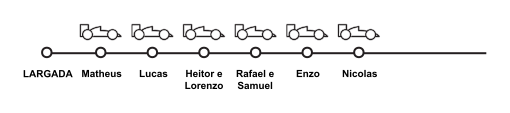
\includegraphics[width=95mm, keepaspectratio]{../../livro/media/cap2/secoes/pngs_licao_02/ativ12_resposta.png}

\end{resposta*}



\subsection{Atividade 13}





  \noindent {\bf Objetivo específico: Levar o aluno a}\vspace{.1cm}:

  \begin{itemize} %s
    \item       Perceber que uma mesma fração (no caso, $\frac{1}{2}$) de unidades diferentes pode resultar em quantidades diferentes.
\end{itemize} %s


  \vspace{.1cm} 
  
  \noindent {\bf Recomendações e sugestões para o desenvolvimento da atividade:}\vspace{.1cm}

  \begin{itemize} %s
    \item       Esta é uma atividade que o aluno pode fazer individualmente, mas é essencial que seja discutida com toda a turma.
    \item       No final da atividade, é importante enfatizar para seus alunos a propriedade matemática que esta atividade quer destacar, ou seja, que uma mesma fração de unidades diferentes pode resultar em quantidades diferentes. Observe para eles que, no contexto       ``frações de''      , é fundamental saber a que o       ``de''       se refere, isto é, qual é a unidade que está sendo considerada. Neste sentido, esta atividade está fortemente relacionada com a Atividade 8.
\end{itemize} %s


  Classificações
\begin{itemize} %s
    \item       Heid et al.: Raciocínio: corroborar
    \item       Nicely, Jr.: Nível 6: justificar
    \item       UERJ: Analisar: levantar hipóteses
\end{itemize} %s


\begin{resposta*}{Atividade 13}
  José está certo se a pizza da qual comeu metade for maior do que a pizza da qual Ella comeu metade, como ilustra a figura a seguir.
  \begin{center}
   \begin{tikzpicture}[x=1mm,y=1mm]
    \draw (0,0) circle (4);
    \draw[fill=attention] (90:4) arc (90:270:4) --  cycle;
    \draw[fill=common, fill opacity=.3] (90:4) arc (90:-90:4) --  cycle;
    \node at (0,8) {Pizza de Ella};
    \begin{scope}[shift={(20,0)}]
    \draw (0,0) circle (8);
    \draw[fill=attention] (90:8) arc (90:270:8) --  cycle;
    \draw[fill=common, fill opacity=.3] (90:8) arc (90:-90:8) --  cycle;
    \node at (0,12) {Pizza de José};
    \end{scope}
   \end{tikzpicture}

  \end{center}

  \end{resposta*}



\subsection{Atividade 14}




  \noindent {\bf Objetivo específico: Levar o aluno a}\vspace{.1cm}

  \begin{itemize} %s
    \item       Analisar uma situação envolvendo frações em representação por meio de figuras cujas repartição não identfica explicitamente o denominador da fração.
\end{itemize} %s


  \vspace{.1cm} 
  
  \noindent {\bf Recomendações e sugestões para o desenvolvimento da atividade:}\vspace{.1cm}
  
\begin{itemize} %s
    \item       Esta é uma atividade que o aluno pode fazer individualmente, mas é essencial que seja discutida com toda a turma.
    \item       No final da atividade, é importante enfatizar para seus alunos a questão matemática que esta atividade quer destacar, ou seja, que o fato de uma figura estar divida em 5 partes e 3 delas estarem pintadas de vermelho,       {\bf não necessariamente implica}       que a parte pintada é       $\frac{3}{5}$       da figura.
    \item       O tipo de situação descrita na atividade é um equívoco comum entre os alunos, isto é, eles equivocamente contam partes sem o cuidado de verificar se as partes nas quais a unidade está dividida correspondem a uma mesma quantidade.
\end{itemize} %s


  Classificações
\begin{itemize} %s
    \item       Heid et al.: Raciocínio: corroborar
    \item       Nicely, Jr.: Nível 9: avaliar
    \item       UERJ: Avaliar: julgar
\end{itemize} %s



\begin{resposta*}{Atividade 14}
  Miguel está equivocado: a parte pintada da figura   {\bf não}   corresponde a   $\frac{3}{5}$   da figura porque a figura não está dividida em 5 partes iguais, ou seja, a figura não está equiparticionada em 5 partes para que as 3 partes pintadas correspondam a   $\frac{3}{5}$   da mesma. Outra justificativa possível é: partindo-se a parte pintada em 3 partes iguais e justapondo-se 5 cópias de uma destas partes, pode-se recompor a figura apenas parcialmente.

\end{resposta*}



\subsection{Atividade 15}



  \noindent {\bf Objetivo específico: Levar o aluno a}\vspace{.1cm}

  \begin{itemize} %s
    \item       Perceber que se uma unidade foi dividida em       $n + m$       partes iguais, das quais       $n$       foram pintadas, então       $\frac{n}{m}$             {\bf não especifica}       a fração da unidade que foi pintada.
\end{itemize} %s


  \vspace{.1cm} 
  
  \noindent {\bf Recomendações e sugestões para o desenvolvimento da atividade:}\vspace{.1cm}
  
\begin{itemize} %s
    \item       Esta é uma atividade que o aluno pode fazer individualmente, mas é essencial que seja discutida com toda a turma.
    \item       O tipo de situação descrita na atividade é um equívoco comum entre os alunos. Assim, esta atividade é uma oportunidade para reforçar os papeis do denominador e do numerador na notação simbólica matemática para frações: o denominador especifica o número de partes iguais na qual a unidade foi dividida e o numerador especifica o número de cópias que foram tomadas de uma destas partes.
\end{itemize} %s


  Classificações
\begin{itemize} %s
    \item       Heid et al.: Raciocínio: corroborar
    \item       Nicely, Jr.: Nível 9: avaliar
    \item       UERJ: Avaliar: julgar
\end{itemize} %s


\begin{resposta*}{Atividade 15}
  A parte pintada de vermelho   {\bf não}   corresponde a   $\frac{3}{4}$   da figura. Ela corresponde a   $\frac{3}{7}$   da figura. De fato: a figura foi dividida em   $7$   partes iguais das quais   $3$   foram pintadas.
\end{resposta*}



\subsection{Atividade 16}



  \noindent {\bf Objetivo específico: Levar o aluno a}\vspace{.1cm}
  
\begin{itemize} %s
    \item       Perceber a importância da explicitação unidade na representação de quantidades.
\end{itemize} %s


  \vspace{.1cm} 
  
  \noindent {\bf Recomendações e sugestões para o desenvolvimento da atividade:}\vspace{.1cm}
  
\begin{itemize} %s
    \item       Esta é uma atividade que o aluno pode fazer individualmente, mas é essencial que seja discutida com toda a turma.
    \item       Recomenda-se que os itens da atividade sejam feitos e corrigidos um a um, de forma a permitir que um aluno que tenha errado um item possa acertar o seguinte.
    \item       O fato de a unidade não estar clara, torna ambígua a questão. É importante que os alunos percebam que, por exemplo, no item a), se a unidade considerada for um dos hexágonos, a fração correspondente a região em vermelho é $\frac{1}{2}$. No entanto, se forem os dois hexágonos, é $\frac{1}{4}$.
    \item       No final de cada item da atividade, é importante enfatizar para seus alunos a propriedade matemática que esta atividade quer destacar, ou seja, que uma mesma quantidade pode ser expressa por frações diferentes dependendo da unidade escolhida. Observe para eles que, no contexto       ``frações de''      , é fundamental saber a que o       ``de''       se refere, isto é, qual é a unidade que está sendo considerada. Neste sentido, esta atividade está fortemente relacionada com as Atividades 8 e 13. Ela também é uma preparação para a Atividade 17, onde a mesma questão é posta, mas agora com um modelo mais comumente usado e, portanto, mais resistente à reflexão que se deseja estabelecer.
\end{itemize} %s


  Classificações
\begin{itemize} %s
    \item       Heid et al.: Raciocínio: corroborar
    \item       Nicely, Jr.: Nível 9: avaliar
    \item       UERJ: Avaliar: julgar
\end{itemize} %s

\def \tripinha{ (30:4) -- (90:4) -- (150:4)--(210:4)--(270:4)--(330:4) [shift={({4*sqrt(3)},0)}] --(270:4) -- (330:4) -- (30:4) -- (90:4)--(150:4)--cycle;}


\def \tripa{ (30:4) -- (90:4) -- (150:4)--(210:4)--(270:4)--(330:4) [shift={({4*sqrt(3)},0)}] --(270:4) -- (330:4) [shift={({4*sqrt(3)},0)}]--  (270:4) -- (330:4) -- (30:4) -- (90:4)--(150:4) [shift={({-4*sqrt(3)},0)}] -- (90:4) -- (150:4)--cycle;}

\def \tripalonga{ (30:4) -- (90:4) -- (150:4)--(210:4)--(270:4)--(330:4) [shift={({4*sqrt(3)},0)}] --(270:4) -- (330:4) [shift={({4*sqrt(3)},0)}] --(270:4) -- (330:4)[shift={({4*sqrt(3)},0)}] --(270:4) -- (330:4) [shift={({4*sqrt(3)},0)}]--  (270:4) -- (330:4) -- (30:4) -- (90:4)--(150:4) [shift={({-4*sqrt(3)},0)}] -- (90:4) -- (150:4)[shift={({-4*sqrt(3)},0)}] -- (90:4) -- (150:4) [shift={({-4*sqrt(3)},0)}] -- (90:4) -- (150:4)--cycle;}

\begin{resposta*}{Atividade 16}

\begin{enumerate} [\quad a)] %s
    \item       A parte em vermelho pode representar       $\frac{1}{2}$       ou       $\frac{1}{4}$       dependendo da unidade, que não foi explicitada no enunciado. Se, por exemplo, a unidade for
    \begin{tikzpicture}[x=1mm,y=1mm]
     \draw[fill=common, fill opacity=.3] (0:4) -- (60:4)--(120:4)-- (180:4)--(240:4)--(300:4)--cycle;     
    \end{tikzpicture}
 então a parte pintada de vermelho em  \begin{tikzpicture}[x=1mm,y=1mm]
 \draw[fill=common, fill opacity=.3] \tripinha;
\begin{scope}
 \clip \tripinha;
\draw[fill=attention] (-4,-4) rectangle (0,4);
\end{scope}
\end{tikzpicture} 
é   $\frac{1}{2}$   desta unidade. Por outro lado,  se a unidade for   \begin{tikzpicture}[x=1mm,y=1mm]
                                                                        \draw[fill=common, fill opacity=.3] \tripinha
                                                                       \end{tikzpicture}
   então a parte pintada de vermelho em  \begin{tikzpicture}[x=1mm,y=1mm]
 \draw[fill=common, fill opacity=.3] \tripinha;
\begin{scope}
 \clip \tripinha;
\draw[fill=attention] (-4,-4) rectangle (0,4);
\end{scope}
\end{tikzpicture}    é   $\frac{1}{4}$   desta unidade.

    \item       A parte em vermelho pode representar       $\frac{1}{2}$       ou       $\frac{3}{2}$       dependendo da unidade, que não foi explicitada no enunciado. Se, por exemplo, a unidade for \begin{tikzpicture}[x=1mm,y=1mm] \draw[fill=common, fill opacity=.3] \tripa  \end{tikzpicture} então a parte pintada de vermelho em \begin{tikzpicture}[x=1mm,y=1mm]
 \draw[fill=common, fill opacity=.3] \tripa;
\begin{scope}
 \clip \tripa;
\draw[fill=attention] (-4,-4) rectangle ({4*sqrt(3)},4);
\end{scope}
\end{tikzpicture} 
   é   $\frac{1}{2}$   desta unidade. Por outro lado,  se a unidade for  \begin{tikzpicture}[x=1mm,y=1mm]
     \draw[fill=common, fill opacity=.3] (0:4) -- (60:4)--(120:4)-- (180:4)--(240:4)--(300:4)--cycle;     
    \end{tikzpicture}  então a parte pintada de vermelho em   
    \begin{tikzpicture}[x=1mm,y=1mm]
    \draw[fill=common, fill opacity=.3] \tripa;
    \begin{scope}
    \clip \tripa;
    \draw[fill=attention] (-4,-4) rectangle ({4*sqrt(3)},4);
    \end{scope}
    \end{tikzpicture}    é   $\frac{3}{2}$   desta unidade.

    \item       A parte em vermelho pode representar       $\frac{3}{5}$       ou       $3$       dependendo da unidade, que não foi explicitada no enunciado. Se, por exemplo, a unidade for \begin{tikzpicture}[x=1mm,y=1mm] \draw[fill=common, fill opacity=.3] \tripalonga  \end{tikzpicture} então a parte pintada de vermelho em \begin{tikzpicture}[x=1mm,y=1mm]
 \draw[fill=common, fill opacity=.3] \tripalonga;
\begin{scope}
 \clip \tripalonga;
  \draw[fill=attention] (-4,-4) rectangle ({10*sqrt(3)},4);
\end{scope}
\end{tikzpicture} 
  é   $\frac{3}{5}$   desta unidade. Por outro lado,  se a unidade for \begin{tikzpicture}[x=1mm,y=1mm]
     \draw[fill=common, fill opacity=.3] (0:4) -- (60:4)--(120:4)-- (180:4)--(240:4)--(300:4)--cycle;     
    \end{tikzpicture} então a parte pintada de vermelho em \begin{tikzpicture}[x=1mm,y=1mm]
 \draw[fill=common, fill opacity=.3] \tripalonga;
\begin{scope}
 \clip \tripalonga;
  \draw[fill=attention] (-4,-4) rectangle ({10*sqrt(3)},4);
\end{scope}
\end{tikzpicture} é   $3$   desta unidade.
\end{enumerate} %s
\end{resposta*}

\subsection{Atividade 17}



  \noindent {\bf Objetivo específico: Levar o aluno a}\vspace{.1cm}
  
\begin{itemize} %s
    \item       Perceber a importância da unidade na representação de quantidades.
\end{itemize} %s



  \vspace{.1cm} 
  
  \noindent {\bf Recomendações e sugestões para o desenvolvimento da atividade:}\vspace{.1cm}
  
\begin{itemize} %s
    \item       Esta é uma atividade que o aluno pode fazer individualmente, mas é essencial que seja discutida com toda a turma.
    \item       No final da atividade, é importante enfatizar para seus alunos a propriedade matemática que esta atividade quer destacar, ou seja, que uma mesma quantidade pode ser expressa por frações diferentes dependendo da unidade escolhida. Observe para eles que, no contexto       ``frações de''      , é fundamental saber a que o       ``de''       se refere, isto é, qual é a unidade que está sendo considerada. Neste sentido, esta atividade está fortemente relacionada com as Atividades 8 e 13.
\end{itemize} %s


  Classificações
\begin{itemize} %s
    \item       Heid et al.: Raciocínio: corroborar
    \item       Nicely, Jr.: Nível 9: avaliar
    \item       UERJ: Avaliar: julgar
\end{itemize} %s


\begin{resposta*}{Atividade 17}
  As afirmações de Júlia, David e Laura estão incompletas, pois ao especificarem as frações   $\frac{3}{5}$  ,   $\frac{3}{2}$   e   $\frac{3}{1}$  , eles não informaram a   {\bf unidade}   a qual estas frações se referem. Desta maneira, não é possível decidir quem está certo. De fato, dependendo da escolha da unidade, cada um deles pode estar certo e os demais errados. Por exemplo, se a unidade for
\begin{center}
  \begin{tikzpicture}[x=1mm,y=1mm]
 \draw[fill=common, fill opacity=.3, scale=4] (0,0) rectangle (5,3);
\end{tikzpicture}
\end{center}
então a parte pintada de vermelho em 
\begin{center}
\begin{tikzpicture}[x=1mm,y=1mm]
 \draw[fill=attention, scale=4] (0,0) rectangle (3,3);
 \draw[fill=common, fill opacity=.3, scale=4] (3,0) rectangle (5,3);
 \foreach \x in {1,2,4} \draw[scale=4] (\x,0) -- (\x,3); 
\end{tikzpicture}
\end{center}
de fato corresponde a   $\frac{3}{5}$   desta unidade, de modo que, nesta situação, Júlia está certa e David e Laura estão errados. Contudo, se a unidade for
\begin{center}
\begin{tikzpicture}[x=1mm,y=1mm]
 \draw[fill=common, fill opacity=.3, scale=4] (0,0) rectangle (2,3);
\end{tikzpicture}
\end{center}
então a parte pintada de vermelho em
\begin{center}
\begin{tikzpicture}[x=1mm,y=1mm]
 \draw[fill=attention, scale=4] (0,0) rectangle (3,3);
 \draw[fill=common, fill opacity=.3, scale=4] (3,0) rectangle (5,3);
 \foreach \x in {1,2,4} \draw[scale=4] (\x,0) -- (\x,3); 
\end{tikzpicture}
\end{center}
  corresponde a   $\frac{3}{2}$   desta unidade,  de modo que, nesta situação, David está certo e Júlia e Laura estão errados. Finalmente, se a unidade for
\begin{center}
\begin{tikzpicture}[x=1mm,y=1mm]
 \draw[fill=common, fill opacity=.3, scale=4] (0,0) rectangle (1,3);
\end{tikzpicture}
\end{center}
então a parte pintada de vermelho em
\begin{center}
\begin{tikzpicture}[x=1mm,y=1mm]
 \draw[fill=attention, scale=4] (0,0) rectangle (3,3);
 \draw[fill=common, fill opacity=.3, scale=4] (3,0) rectangle (5,3);
 \foreach \x in {1,2,4} \draw[scale=4] (\x,0) -- (\x,3); 
\end{tikzpicture}
\end{center}
  corresponde a   $3$   desta unidade e, neste caso, Laura está certa e David e Júlia estão errados.
\end{resposta*}

\subsection{Atividade 18}

{\bf Objetivos da Atividade:}\vspace{.1cm}

\begin{itemize} %s
    \item       Relembrar divisão com resto (ou divisão euclidiana).
    \item       Selecionar, dentro de uma situação plausível do dia a dia, dados relevantes para resolver um problema.
\end{itemize} %s
\vspace{.1cm}

{\bf Observações para o professor:}\vspace{.1cm}

\begin{itemize} %s
    \item       A atividade deve ser conduzida de forma a chegar-se na divisão euclidiana. Ou seja, o aluno pode começar montando as pizzas (tanto na proposta digital como com material concreto). Se não for possível oferecer a atividade na forma digital, recomenda-se que os alunos tenham à mão o material concreto: fatias de pizza cortadas em papel ou em E.V.A..
    \item       É possível que os alunos resolvam o item (a) a partir da divisão euclidiana, efetuando a divisão de 38 por 8: 38 = 4 x 8 + 6. Se esse for o caso, recomenda-se que o professor, destaque a informação associada a cada um dos números na expressão. Em particular o       ``resto''      , que identifica uma quantidade menor do que uma pizza (resto 6 indica 6 fatias, que é menor do que uma pizza, uma vez que cada pizza tem 8 fatias).
    \item       Para responder ao item (b), o aluno deve reconhecer que cada fatia é igual a       $\frac{1}{8}$       da pizza. Poranto, a quantidade total de pizza consumida pelos amigos pode ser expressa como       $\frac{38}{8}$       de uma pizza. Cabe destacar que essa fração corresponde a 4 pizzas +       $\frac{6}{8}$       de uma pizza.
    \item        Observe que, neste contexto, o resto, que é um número inteiro representando o número de fatias, também pode ser expresso por meio de uma fração da unidade pizza:       $\frac{6}{8}$       de uma pizza.
    \item       Faz parte da atividade a tarefa de selecionar dados relevantes para o problema, o que a torna um tanto complexa, por isso é a última Atividade da Lição 2. Para os itens (a) e (b), a quantidade de amigos, 7, é irrelevante. No entanto, é relevante para o ítem (c ).
    \item       A atividade tem também o objetivo de evidenciar que, no dia a dia, nem toda partição é uma equipartição: 38 fatias de pizza para 7 amigos é um exemplo.
\end{itemize} %s



\begin{resposta*}{Atividade 18}
\begin{enumerate} [\quad a)] %s
    \item       A solução corresponde ao quociente da divisão euclidiana de 38 por 8: 4
    \item       Compreendendo que cada fatia é       $\frac{1}{8}$        de uma pizza: 4 pizzas e       $\frac{6}{8}$       ou       $\frac{38}{8}$      .
    \item       A divisão euclidiana de 38 por 7 fornece um resto diferente de zero, o que indica que não é possível que todos os amigos tenham comido o mesmo número de fatias de pizza, ou, a mesma quantidade de pizza.
\end{enumerate} %s
\end{resposta*}


\end{multicols}
